\documentclass[]{article}
\usepackage[T1]{fontenc}
\usepackage{amsfonts}
\usepackage{amsmath} 
\usepackage{graphicx}
\usepackage{float}
\usepackage{longtable}
\usepackage[polish]{babel} % English language/hyphenation
\usepackage[linesnumbered,lined,boxed,commentsnumbered,ruled,vlined]{algorithm2e}


% klikalny spis treści

\usepackage{color}
\usepackage{hyperref}
\hypersetup{
	colorlinks,
	citecolor=black,
	filecolor=black,
	linkcolor=mypink1  ,
	urlcolor=black
}


\graphicspath{ {img/} }

%opening
\title{Projekt Zespołowy \\
	\Huge Etap projektu – projektowanie rozwiązania na zadaną architekturę}
\author{\\ \\ \\ Autorzy:
	\\Biernacka Kamila\\ 
	Kania Dominik\\ 
	Leśniak Mateusz\\ 
	Maziarz Wojciech\\ \\ \\ \\ \\ \\ \\ \\ \\ \\ \\ \\ \\ \\ \\ \\ \\  }
\date{kwiecień 2021}

\begin{document}
\definecolor{mypink1}{rgb}{0.858, 0.188, 0.478}



\maketitle
\newpage



\begin{abstract}
Poniższe sprawozdanie jest wynikiem pracy na drugim etapie projektu zespołowego z implementacji metody indeksu w architekturach GPU. Przedstawiono w nim przygotowane przez zespół projekty i rysunki koncepcyjne wymaganych do zaimplementowania algorytmów.
\end{abstract}

\tableofcontents
\clearpage
\section{Oznaczenia} ~


\begin{longtable}{|p{.2\textwidth}|l|}
	\caption{Oznaczenia funkcji i operatorów. \textit{Źródło: opracowanie własne}}
	\label{oznaczenia}
	\\\hline
	\textbf{Symbol}   & 	\textbf{Opis} \\ \hline
	$>>$& przesunięcie bitowe\\ \hline
	$\&\&$     & koniunkcja bitowa\\ \hline
	$\%$  & reszta z dzielenia \\ \hline
	\texttt{to\_bin()}  & zwraca postać binarną argumentu \\ \hline
	\texttt{length()}  & zwraca długość argumentu \\ \hline
	\texttt{randomInt()} & zwraca losową liczbę całkowitą \\ \hline
	\texttt{swap(a,b)} & zmiennej a przypisuje wartość zmiennej b i odwrotnie\\ \hline
	
\end{longtable}
\newpage

\section{Mnożenie modularne dużych liczb}
	W celu wykonania mnożenia dużych liczb \(a, b \in \mathbb{F}_p\) wykorzystany zostanie algorytm \ref{mult}.
	Pierwszym krokiem jest przedstawienie liczb \(a, b\) w postaci \(a = x_1 \cdot 2^{32} + y_1\) oraz 
	\(b = x_2 \cdot 2^{32} + y_2\).
	\newline
	Wtedy
	\newline
	\(r_p = r_p(ab) = r_p((x_1 \cdot 2^{32} + y_1)(x_2 \cdot 2^{32} + y_2)) = r_p(x_1x_2 \cdot_p 2^{64}) +_p r_p(x_1y_2 \cdot_p 2^{32}) +_p r_p(x_2y_1 \cdot_p 2^{32}) +_p r_p(y_1y_2)\).
	\newline 
	Do wyznaczenia pośrednich wartości \(r_p\) wykorzystywany jest algorytm \ref{half_mult}. Algorytm mnożenia pośredniego działa analogicznie do algorytmu \ref{mult}. Różnicą jest przedstawienie czynników jako \(x \cdot 2^{16} + y\).
	\newline
	\begin{algorithm}[H]
		\SetAlgoLined
		\caption{Mnożenie pośrednie, \texttt{halfMult}}
		\label{half_mult}
		\KwIn{\(a,b\) - dwie liczby całkowite, \(p\) - modulnik}
		\KwOut{\(result\) - wynik mnożenia}
		\(x_1 \gets a >> 16\)\\
		\(y_1 \gets a \; \&\& \; 0xffff \) \\
		\(x_2 \gets b >> 16\)\\
		\(y_2 \gets b \; \&\& \; 0xffff \) \\
		\(half_a \gets (((x_1 x_2) \% p) \cdot r_p(2^{32})) \%p\) \\
		\(half_b \gets (((x_1 y_2) \% p) \cdot r_p(2^{16})) \%p\) \\
		\(half_c \gets (((x_2 y_1) \% p) \cdot r_p(2^{16})) \%p\) \\
		\(half_d \gets (y_1 y_2) \%p\) \\
		\Return{\((half_a + half_b + half_c + half_d) \% p\)}
	\end{algorithm}

	
	\begin{algorithm}[H]
		\SetAlgoLined
		\caption{Pełne mnożenie modularne dwóch liczb, \texttt{mult}}
		\label{mult}
		\KwIn{\(a,b\) - dwie liczby całkowite, \(p\) - modulnik}
		\KwOut{\(result\) - wynik mnożenia}
		\(x_1 \gets a >> 32\)\\
		\(y_1 \gets a \; \&\& \; 0xffffffff \) \\
		\(x_2 \gets b >> 32\)\\
		\(y_2 \gets b \; \&\& \; 0xffffffff \) \\
		\(half_a \gets (halfMult(x_1, x_2) \cdot r_p(2^{64})) \% p\) \\
		\(half_b \gets (halfMult(x_1, y_2) \cdot r_p(2^{32})) \% p\) \\
		\(half_c \gets (halfMult(x_2, y_1) \cdot r_p(2^{32})) \% p\) \\
		\(half_a \gets halfMult(y_1, y_2)\) \\
		\Return{\((half_a + half_b + half_c + half_d) \% p\)}
	\end{algorithm}
	
\newpage
\section{Poszukiwanie relacji i faktoryzacja w bazie}
	\subsection{Szybkie potęgowanie modularne}
	Metoda indeksu wymaga obliczenia wartości typu $a^{b}\;{mod}\;n$.
	Szybkie potęgowanie modularne jest prostym algorytmem pozwalającym zredukować liczbę mnożeń i dzieleń modulo z $b$ do \textit{O(log b)}.
	\newline
	\begin{algorithm}[H]
		\caption{Szybkie potęgowanie modularne,  \texttt{fastPow}} 
		\label{szybkie_pot} 
		\SetKwInOut{Input}{Input}\SetKwInOut{Output}{Output}
		\Input{podstawa potęgi $a$, wykładnik potęgi $b$, modulnik $n$}
		\Output{$a^{b}\;mod\;n$}
		\BlankLine
		$bits \gets to\_bin(b)$\\
		$nbits \gets length(bits)$\\
		$a \gets a\%n$\\
		$result \gets 1$\\
		$x \gets a$\\
		\For{i \(\gets\) 0 \textbf{to} nbits}{
			\If{bits[i]==1}{
				$result \gets result*x$\\
				$result \gets result\%n$\\
			}
			$x \gets x*x$\\
			$x \gets x\%n$\\
		}
		\Return{$result$}
	\end{algorithm}

	\begin{figure}[H]
		\begin{center}
			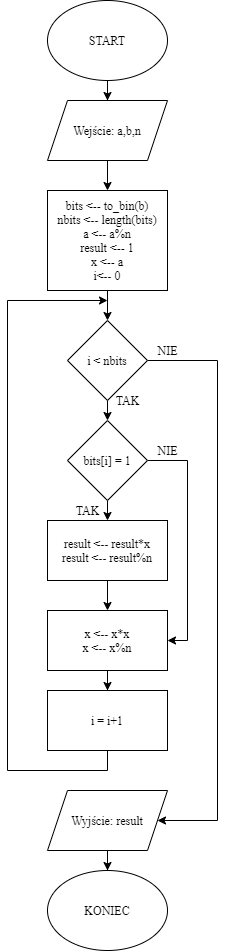
\includegraphics[width=4.5cm]{alg 3.png} \caption{Schemat blokowy algorytmu \ref{szybkie_pot}}
		\end{center}
	\end{figure}
	
	\subsection{Faktoryzacja w bazie}
		Dana jest baza \(\mathcal{N} = \{2, 3, \dots p_k\}\), gdzie \(p_i \in \mathcal{P}\) i \(p_k\) jest największą liczbą pierwszą mniejszą \(B\). 
		W celu faktoryzacji wykorzystany zostanie algorytm \ref{factor}.
		\newline
		\begin{algorithm}[H]
			\SetAlgoLined
			\caption{Faktoryzacja w bazie, \texttt{factor}}
			\label{factor}
			\KwIn{\(a\) - faktoryzowana liczba, \(\mathcal{N}\) - baza rozkładu}
			\KwOut{\(result = [e_1, e_2, \dots, e_k]\) - czynniki}
			\For{\(i \gets 0\) \textbf{to} \(k\)}
			{
				\(counter \gets 0\) \\
				\While{\(a \% N[i]\)}
				{
					\(a \gets \frac{a}{N[i]}\) \\
					\(counter \gets counter + 1\) \\
				}
				\(result[i] \gets counter\) \\
			}
			\Return{\(result\)}
		\end{algorithm}
\clearpage
		\begin{figure}[H]
			\begin{center}
				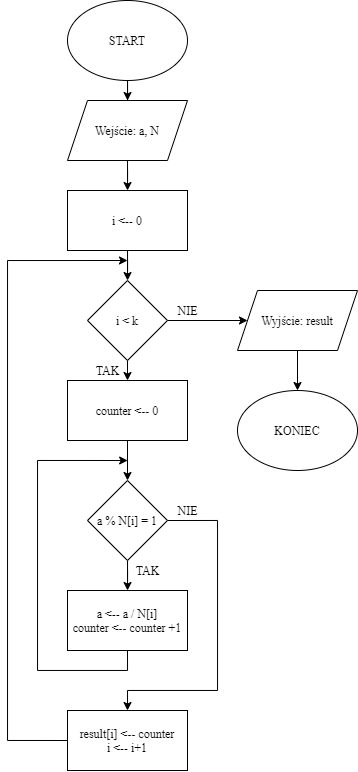
\includegraphics[width=8cm]{alg 4.png} \caption{Schemat blokowy algorytmu \ref{factor}}
			\end{center}
		\end{figure}
	
		\begin{algorithm}[H]
			\SetAlgoLined
			\caption{Sprawdzenie czy liczba faktoryzuje się w wybranej bazie, \texttt{IsFactored}}
			\label{factor_alt}
			\KwIn{\(a\) - faktoryzowana liczba, \(\mathcal{N}\) - baza rozkładu}
			\KwOut{\(result = [e_1, e_2, \dots, e_k]\) - czynniki}
			\For{\(i \gets 0\) \textbf{to} \(k\)}
			{
				\(counter \gets 0\) \\
				\While{\(a \% N[i]\)}
				{
					\(a \gets \frac{a}{N[i]}\) \\
					\(counter \gets counter + 1\) \\
				}
				\(result[i] \gets counter\) \\
			}
			\If{\(a == 1\)}
			{
				\Return{\(True\)}
			}
			\Else
			{
				\Return{\(False\)}
			}
			
		\end{algorithm}
	
		\begin{figure}[H]
			\begin{center}
				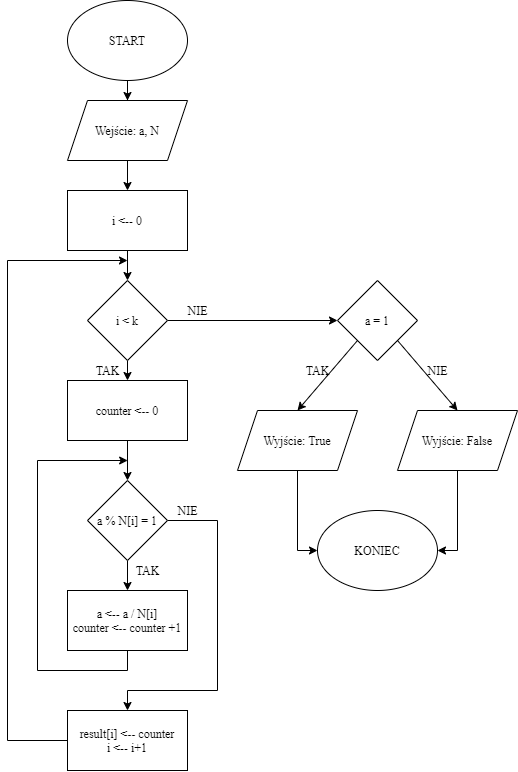
\includegraphics[width=10cm]{alg 5.png} \caption{Schemat blokowy algorytmu \ref{factor_alt}}
			\end{center}
		\end{figure}
	
	
\clearpage
	\subsection{Budowa relacji}
		W celu zbudowania relacji \(\mathcal{R}\) generowanych jest \(l\) liczb losowych \(e_i\). Następnie, przy wykorzystaniu algorytmu \ref{szybkie_pot}, wyznaczane są wartości \(a^{e_i}\). 
		\newline
		Niech \(e\) będzie tablicą \(l\)- elementową, jako \(fastPow(a, e, p)\) rozumiane jest jednoczesne wykonanie \(fastPow(a, e_i, p)\) dla każdego elementu tablicy z wykorzystaniem procesora graficznego. 
		\newline
		\begin{algorithm}[H]
			\SetAlgoLined
			\caption{Budowa relacji, \texttt{relationBuild}}
			\label{relation}
			\KwIn{\(a\) - generator, \(l\) - wielkość zbioru relacji, \(p\) - modulnik}
			\KwOut{\(R\) - zbiór relacji}
			\For{\(i \gets 0\) \textbf{to} \(l\)}
			{
				\(e[i] \gets randomInt()\)
			}
			\(R \gets fastPow(a, e, p)\) \\
			\For{\(i \gets 0\) \textbf{to} \(l\)}
			{
				\While{ \textbf{not} \(isFactored(R[i])\)}
				{
					\(R[i] \gets fastPow(a, randomInt(), p)\)
				}
			}
		
			\Return{\(R\)}
		\end{algorithm}

\clearpage
	\begin{figure}[H]
		\begin{center}
			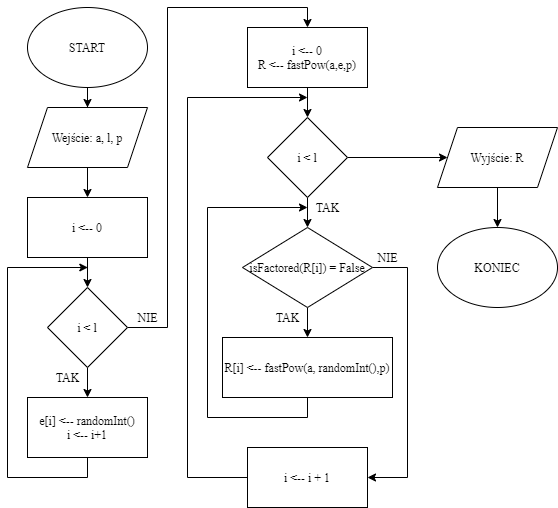
\includegraphics[width=13cm]{alg 6.png} \caption{Schemat blokowy algorytmu \ref{relation}}
		\end{center}
	\end{figure}

\newpage
\section{Eliminacja Gaussa w pierścieniu \(\mathbb{Z}_{p-1}\)}
	\subsection{Algorytm Euklidesa}
		Poniższy schemat wykorzystuje algorytm Euklidesa do sprawdzenia, czy podane na wejściu dwie liczby są względnie pierwsze. \\
	\begin{algorithm}[H]
		\label{Euklid}
		\caption{Algorytm Euklidesa, \texttt{isInversible}}
		\KwIn{$a, b$ - liczby naturalne}
		\KwOut{True, jeśli $\gcd(a,b) == 1$, False w przeciwnym przypadku.}
		\BlankLine
		\While{$b \neq 0$}{
			$temp \gets b$ \\
			$b \gets a$ mod $  b$ \\
			$a \gets temp$} 
		\If{$a == 1$}{\Return{\(True\)} }
		\Else{\Return{\(False\)}}
		
	\end{algorithm}

	\begin{figure}[H]
		\begin{center}
			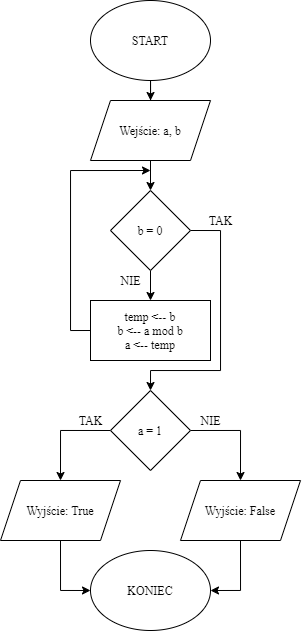
\includegraphics[width=8cm]{alg 7.png} \caption{Schemat blokowy algorytmu \ref{Euklid}}
		\end{center}
	\end{figure}

	\subsection{Rozszerzony algorytm Euklidesa}
		Tożsamość Bezout mówi, że liczby $a$ i $p$ są względnie pierwsze i wtedy i tylko wtedy, gdy istnieją takie liczby $s$ i $t$, że
		\begin{center}
			$ps + at = 1$,
		\end{center}
		Wówczas, po zredukowaniu tej równości modulo $p$, otrzymuje się
		\begin{center}
			$at \equiv 1$ mod $p$,
		\end{center}
		 czyli $t$ jest elementem odwrotnym $a$ w pierścieniu $Z_{p}$. \\
		Wykorzystując poniższy algorytm możemy znaleźć odwrotność w dowolnym pierścieniu liczbowym.
		
		\begin{algorithm}[H]
			\label{extEuklid}
			\caption{Rozszerzony Algorytm Euklidesa, \texttt{inverse}}
			\KwIn{$a, p$ - liczby naturalne}
			\KwOut{$x = a^{-1}$ mod $p$ lub informacja, że taka liczba nie istnieje}
			\BlankLine
			$u \leftarrow 1, w \leftarrow a, x \leftarrow 0,z \leftarrow p$ \\
			\While{$w \neq 0$}{
				\If{$w < z$}{
					$swap(u, x)$ \\
					$swap(w, z)$
				}
				$q \leftarrow w / z - (w\%z)$ \\
				$u \leftarrow u - q \cdot x$
				$w \leftarrow w - q \cdot z$	
			}
			\If{$z \neq 1$}{\Return{\(None\)}}
			\If{$ x < 0$}{\(x \gets x + p\)}
			\Return{x}	
		\end{algorithm}
	
	\begin{figure}[H]
		\begin{center}
			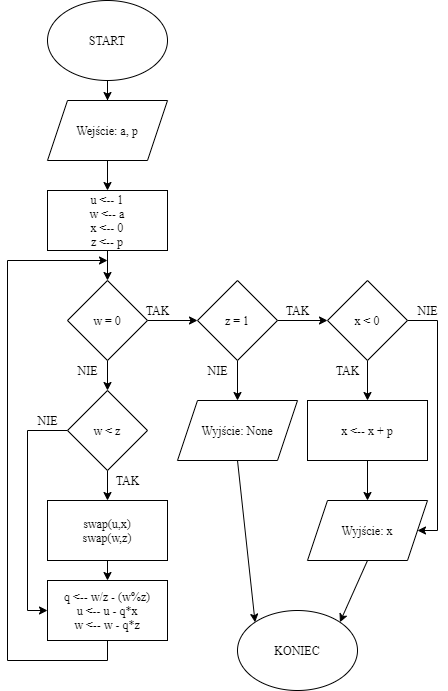
\includegraphics[width=11cm]{alg 8.png} \caption{Schemat blokowy algorytmu \ref{extEuklid}}
		\end{center}
	\end{figure}


	\section{Eliminacja Gaussa}
		Niech 
		\newline
		\begin{center}
			\(\mathbb{A}_{l,k} = 
			\begin{bmatrix}
				a_{0,0} & a_{0,1} & \cdots & a_{0,k} \\
				a_{1,0} & a_{1,1} & \cdots & a_{1,k} \\
				\vdots & \vdots & & \vdots \\
				a_{l,0} & a_{l,1} & \cdots & a_{l,k} 
			\end{bmatrix} \). 
		\end{center}


		Jako \(\mathbb{A}_i = [a_{i,0}, a_{i,1}, \dots, a_{i,k}]\) rozumiany jest \(i\)-wiersz macierzy. Wtedy, następujący zapis \(\mathbb{C} = \mathbb{A}_n - \mathbb{A}_m\), gdzie \(\mathbb{C} = [c_0, c_1, \dots, c_k]\) oznacza jednoczesne wykonanie działania \(c_j = \mathbb{A}_{n,j} - \mathbb{A}_{m,j}\) dla każdego elementu wiersza z wykorzystaniem procesora graficznego. Natomiast \(\mathbb{C} = mult(\mathbb{A}_m, b)\) rozumiany jest jako jednoczesne wykonanie \(mult(a_{m,j}, b)\). Zapis \(\mathbb{A}_{l+1, k} \gets \frac{\mathbb{A}_{l, k}}{vector}\) oznacza dopisanie wiersza \(vector\) jako ostatni wiersz macierzy. 
		\newline
		\begin{algorithm}[H]
			\SetAlgoLined
			\label{Gauss}
			\caption{Algorytm eliminacji Gaussa, \texttt{Gauss}}
			\KwIn{\(\mathbb{A}_{l,k} = \mathbb{A}_{l-1,k} \| \mathbb{E}_{1,k}\)}
			\KwOut{\(\mathbb{X}_{1,k}\)}
			
			\For{\(j \gets 0\) \textbf{to} \(l\)}
			{
				\For{\(i \gets 0\) \textbf{to} \(k\)}
				{
					\If{\(i \neq j\)}
					{
						\(inversibleIdx \gets inversibleIndex(i)\) \\
						\While{\(inversibleIdx == -1 \text{ and } \text{\textbf{not }} isInversible(a_{j,j}) \)}
						{
							\(\mathbb{A}_{l+1, k} \gets \frac{\mathbb{A}_{l, k}}{relationBuild(a, 1, p)} \)\\
							\(l \gets l + 1\) \\
							\(inversibleIdx \gets inversibleIndex(a_i)\) \\
							\(swap(\mathbb{A}_i, \mathbb{A}_{inversibleIdx})\) \\
						}
						\(b \gets mult(a_{i,j}, inverse(a_{j,j}, p-1), p-1)\) \\
						\(tmp \gets mult(\mathbb{A}_i, b, p-1)\) \\
						\(\mathbb{A}_i \gets \mathbb{A}_i - tmp\) \\
					}
				}
			}
			\For{\(i \gets 0\) \textbf{to} \(k\)}
			{
				\(b \gets inverse(a_{i,i}, p-1)\) \\
				\(\mathbb{A}_i \gets mult(\mathbb{A}_i, b, p-1)\) \\
			}
			\Return{\(\mathbb{A}_k\)}
			
		\end{algorithm}
		
				
	\begin{figure}[H]
		\begin{center}
		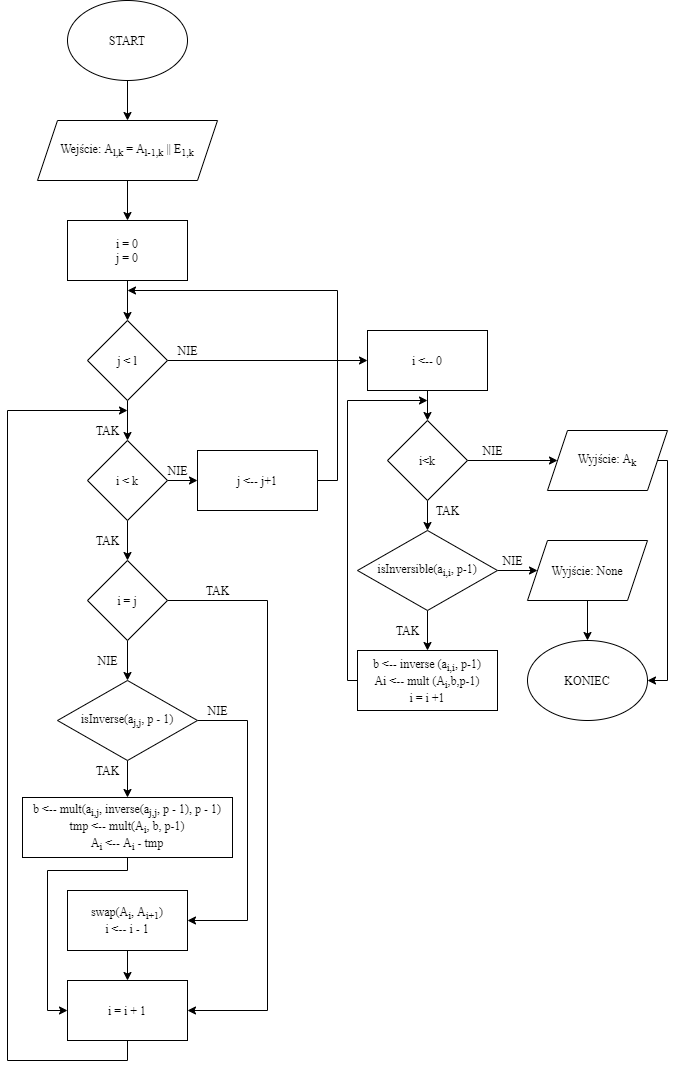
\includegraphics[width = 12cm]{alg9.png} \caption{Schemat blokowy algorytmu \ref{Gauss}}
		\end{center}
	\end{figure}

	
	
\end{document}
